\documentclass[11pt]{standalone}
\usepackage{tikz}
\usetikzlibrary{shapes.geometric}
\usetikzlibrary{arrows.meta,calc,decorations.pathmorphing,shapes.geometric,backgrounds,plotmarks,shapes.multipart}
\begin{document} 
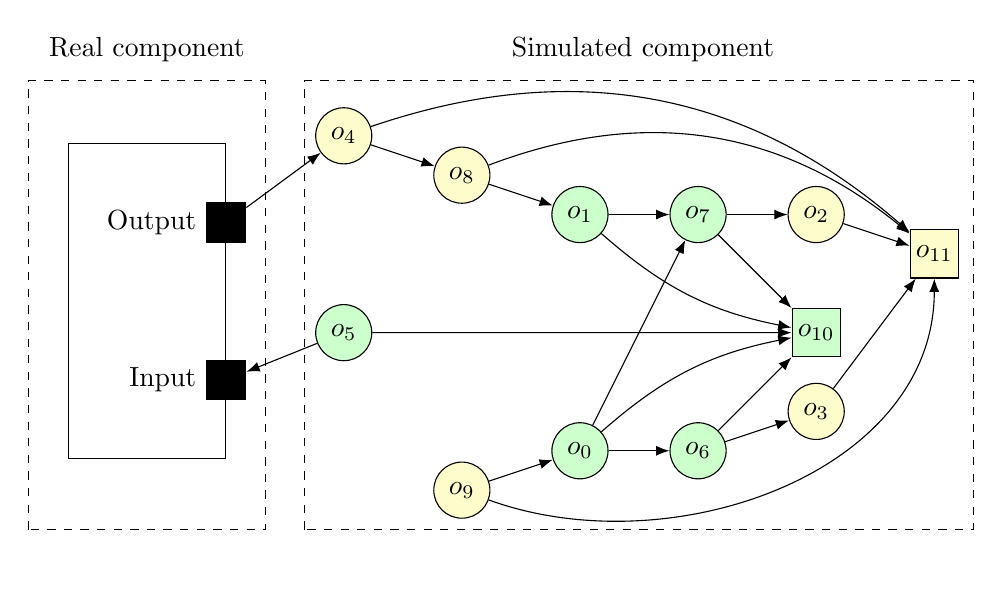
\begin{tikzpicture}
\begin{scope}[framed,local bounding box=scope1,node distance=1.5cm,every node/.style={circle,draw},square/.style={regular polygon,regular polygon sides=4,inner sep=-.5}]

% Nodes
\node[fill=green!20] (o5) {$o_5$};
\node[above of = o5,yshift=1cm,fill=yellow!20] (o4) {$o_4$};
\node[right of = o4,yshift=-.5cm,fill=yellow!20] (o8) {$o_8$};
\node[right of = o8,yshift=-.5cm,fill=green!20] (o1) {$o_1$};
\node[right of = o1,fill=green!20] (o7) {$o_7$};
\node[right of = o7,fill=yellow!20] (o2) {$o_2$};
\node[square,right of = o2,yshift=-.5cm,fill=yellow!20] (o11) {$o_{11}$};
\node[square,below of = o2,fill=green!20] (o10) {$o_{10}$};
\node[below of = o10,yshift=.5cm,fill=yellow!20] (o3) {$o_3$};
\node[left of = o3,yshift=-.5cm,fill=green!20] (o6) {$o_6$};
\node[left of = o6,fill=green!20] (o0) {$o_0$};
\node[left of = o0,yshift=-.5cm,fill=yellow!20] (o9) {$o_9$};

%arcs
\path (o5) edge[-{Latex[]}] (o10);
\path (o4) edge[-{Latex[]}] (o8);
\path (o4) edge[-{Latex[]},bend left=30] (o11);
\path (o8) edge[-{Latex[]}] (o1);
\path (o8) edge[-{Latex[]},bend left=30] (o11);
\path (o1) edge[-{Latex[]}] (o7);
\path (o1) edge[-{Latex[]},bend right=15] (o10);
\path (o7) edge[-{Latex[]}] (o2);
\path (o7) edge[-{Latex[]}] (o10);
\path (o2) edge[-{Latex[]}]  (o11);
\path (o9) edge[-{Latex[]}]  (o0);
\path (o9) edge[-{Latex[]}, out=340,in=270]  (o11);
\path (o0) edge[-{Latex[]}]  (o6);
\path (o0) edge[-{Latex[]},bend left=15]  (o10);
\path (o6) edge[-{Latex[]}]  (o3);
\path (o6) edge[-{Latex[]}]  (o10);
\path (o3) edge[-{Latex[]}]  (o11);
\path (o0) edge[-{Latex[]}]  (o7);

%\coordinate (rectr) at ();

\begin{pgfonlayer}{background} 
 \draw[dashed] ([xshift=-.5cm,yshift=-2.5cm]o5) rectangle ([xshift=.5cm,yshift=2.2cm]o11);
\end{pgfonlayer}

\end{scope}

\begin{scope}[xshift=-2.5cm]
\node[rectangle,draw,minimum height=4cm, minimum width=2cm,yshift=.4cm] (frame){};
\node[rectangle,draw,fill=black,minimum height=.5cm, minimum width=.5cm,yshift=1cm,label=west:Output] at(frame.east) (output){};
\node[rectangle,draw,fill=black,minimum height=.5cm, minimum width=.5cm,yshift=-1cm,label=west:Input] at(frame.east) (input){};

\begin{pgfonlayer}{background}[dashed] 
 \draw[dashed] ([xshift=-.5cm,yshift=-2.9cm]frame.west) rectangle ([xshift=.5cm,yshift=2.8cm]frame.east);
\end{pgfonlayer}

\end{scope}

\path (output) edge[-{Latex[]}]  (o4);
\path (o5) edge[-{Latex[]}]  (input);

\node [above of=frame,yshift=2.2cm] (real) {Real component};
\node [right of=real,xshift=5.3cm] (simulated) {Simulated component};
\end{tikzpicture}
\end{document}